\flushbottom


%% CONTINUE




%%=============================================================================
%%=============================================================================
\chapter{Nonlinear Partial Differential Equations}












\raggedbottom
%%============================================================================
\pagebreak
\flushbottom
\section{Exercises}



%%-----------------------------------------------------------------------------
%%\begin{large}
%%\noindent
%%\textbf{}
%%\end{large}





\begin{Exercise}
  Consider the nonlinear PDE
  \[ 
  u_t + u u_x = 0.
  \]
  The solution $u$ is constant along lines 
  (characteristics) such that $x - u t = k$ for any constant $k$. Thus 
  the slope of these lines will depend on the initial data $u(x,0) = f(x)$. 
  \begin{enumerate} 
  \item 
    In terms of this initial data, write down the 
    equation for the characteristic in the $x,t$ plane which goes
    through the point $(x,t) = (\xi,0)$.
  \item 
    State a criteria on $f$ such that two characteristics will
    intersect at some positive time $t$. Assuming intersections do occur, 
    what is the time of the {\em first} intersection? 
    You may assume that $f$ is everywhere continuous and differentiable. 
  \item 
    Apply this to the case where $f(x) = 1 - \e^{-x^2}$ to indicate 
    where and when a shock will form and sketch (roughly) the solution both 
    before and after this time. 
  \end{enumerate}
\end{Exercise}








%%\phi_t + (1+x)\phi_x + \phi = 0 \quad \mathrm{in} \quad 
\begin{Exercise}
  Solve the equation
  \[ 
  \phi_t + (1+x)\phi_x + \phi = 0 \quad \mathrm{in} \quad 
  -\infty < x < \infty,\ t > 0, 
  \]
  with initial condition $\phi(x,0) = f(x)$.
\end{Exercise}



%%\phi_t + \phi_x + \frac{\alpha \phi}{1+x} = 0 
\begin{Exercise}
  Solve the equation
  \[ 
  \phi_t + \phi_x + \frac{\alpha \phi}{1+x} = 0 
  \]
  in the region $0 < x < \infty$, $t > 0$ with initial condition $\phi(x,0)=0$,
  and boundary condition $\phi(0,t) = g(t)$. [Here $\alpha$ is a positive
  constant.]
\end{Exercise}



%%\phi_t + \phi_x +\phi^2 = 0 
\begin{Exercise}
  Solve the equation
  \[ 
  \phi_t + \phi_x +\phi^2 = 0 
  \]
  in $-\infty < x < \infty$, $t > 0$ with initial condition $\phi(x,0)=f(x)$.
  Note that the solution could become infinite in finite time.
\end{Exercise}



%%c_t + c c_x + \mu c = 0, \qquad -\infty < x < \infty,\ t > 0 
\begin{Exercise}
  Consider
  \[ 
  c_t + c c_x + \mu c = 0, \qquad -\infty < x < \infty,\ t > 0.
  \]
  \begin{enumerate}
    %%
  \item
    Use the method of characteristics to solve the problem with
    \[ 
    c = F(x)\ \mathrm{at}\ t = 0. 
    \]
    ($\mu$ is a positive constant.)
    %%
  \item
    Find equations for the envelope of characteristics in the case $F'(x)<0$.
    %%
  \item
    Deduce an inequality relating $\max |F'(x)|$ and $\mu$ which decides
    whether breaking does or does not occur.
  \end{enumerate}
\end{Exercise}



%%For water waves in a channel the so-called shallow water equations are
\begin{Exercise}
  For water waves in a channel the so-called shallow water equations are
  \begin{gather}
    h_t + (hv)_x = 0 \\
    (hv)_t + \left(hv^2 + \frac{1}{2} gh^2 \right)_x = 0, \ g = \mathrm{constant}.
  \end{gather}
  Investigate whether there are solutions with $v=V(h)$, where $V(h)$ is
  not posed in advance but is obtained from requiring consistency between the
  $h$ equation obtained from (1) and the $h$ equation obtained from (2).

  There will be two possible choices for $V(h)$ depending on a choice of sign.
  Consider each case separately.  In each case fix the arbitrary constant
  that arises in $V(h)$ by stipulating that before the waves arrive, $h$
  is equal to the undisturbed depth $h_0$ and $V(h_0)=0$.

  Find the $h$ equation and the wave speed $c(h)$ in each case.
\end{Exercise}



%%After a change of variables, the chemical exchange equations can be put
\begin{Exercise}
  After a change of variables, the chemical exchange equations can be put
  in the form
  \begin{gather}
    \frac{\partial \rho}{\partial t} + \frac{\partial \sigma}{\partial x} = 0 \\
    \frac{\partial \rho}{\partial t} = \alpha \sigma - \beta \rho - \gamma \rho \sigma; \quad
    \alpha, \beta, \gamma = \mathrm{positive constants.}
  \end{gather}
  \begin{enumerate}
    %%
  \item
    Investigate wave solutions in which $\rho = \rho(X)$, $\sigma=\sigma(X)$,
    $X=x-Ut$, $U=\mathrm{constant}$, and show that $\rho(X)$ must satisfy
    an ordinary differential equation of the form
    \[ \frac{\dd \rho}{\dd X} = \mathrm{quadratic in}\ \rho. \]
    %%
  \item
    Discuss ths ``smooth shock'' solution as we did for a different example
    in class.  In particular find the expression for $U$ in terms of the 
    values of $\rho$ as $X \to \pm \infty$, and find the sign of $d\rho/dX$.
    Check that
    \[ U = \frac{\sigma_2-\sigma_1}{\rho_2-\rho_1} \]
    in agreement with the ``discontinuous theory.''
  \end{enumerate}
\end{Exercise}



%%Find solitary wave solutions for the following equations:
\begin{Exercise}
  Find solitary wave solutions for the following equations:
  \begin{enumerate}
  \item $\eta_t + \eta_x + 6 \eta \eta_x - \eta_{xxt} = 0$. 
    (Regularized long wave or B.B.M. equation)
  \item $u_{tt} - u_{xx} - \left(\frac{3}{2} u^2\right)_{xx} - u_{xxxx}=0$.
    (``Boussinesq'')
  \item $\phi_{tt} - \phi_{xx} + 2 \phi_x \phi_{xt} + \phi_{xx} \phi_t
    - \phi_{xxxx} = 0$. (The solitary wave form is for $u=\phi_x$)
  \item $u_t + 30 u^2 u_1 + 20 u_1 u_2 + 10 u u_3 + u_5 = 0$.
    (Here the subscripts denote $x$ derivatives.)
  \end{enumerate}
\end{Exercise}






\raggedbottom
%%============================================================================
\pagebreak
\flushbottom
\section{Hints}



%%-----------------------------------------------------------------------------
%%\begin{large}
%%\noindent
%%\textbf{}
%%\end{large}




\begin{Hint}
  %% CONTINUE
\end{Hint}




%%\phi_t + (1+x)\phi_x + \phi = 0 \quad \mathrm{in} \quad 
\begin{Hint}
\end{Hint}



%%\phi_t + \phi_x + \frac{\alpha \phi}{1+x} = 0 
\begin{Hint}
\end{Hint}



%%\phi_t + \phi_x +\phi^2 = 0 
\begin{Hint}
\end{Hint}



%%c_t + c c_x + \mu c = 0, \qquad -\infty < x < \infty,\ t > 0 
\begin{Hint}
\end{Hint}



%%For water waves in a channel the so-called shallow water equations are
\begin{Hint}
\end{Hint}



%%After a change of variables, the chemical exchange equations can be put
\begin{Hint}
\end{Hint}



%%Find solitary wave solutions for the following equations:
\begin{Hint}
\end{Hint}









\raggedbottom
%%============================================================================
\pagebreak
\flushbottom
\section{Solutions}



%%-----------------------------------------------------------------------------
%%\begin{large}
%%\noindent
%%\textbf{}
%%\end{large}







\begin{Solution}
  \begin{enumerate} 
  \item 
    \begin{gather*}
      x = \xi + u(\xi,0) t
      \\
      x = \xi + f(\xi) t
    \end{gather*}
  \item 
    Consider two points $\xi_1$ and $\xi_2$ where $\xi_1 < \xi_2$.  Suppose that 
    $f(\xi_1) > f(\xi_2)$.  Then the two characteristics passing through the points
    $(\xi_1,0)$ and $(\xi_2,0)$ will intersect.  
    \begin{gather*}
      \xi_1 + f(\xi_1) t = \xi_2 + f(\xi_2) t
      \\
      t = \frac{\xi_2 - \xi_1}{f(\xi_1) - f(\xi_2)}
    \end{gather*}
    We see that the two characteristics intersect at the point
    \[
    (x,t) = \left( \xi_1 + f(\xi_1) \frac{\xi_2 - \xi_1}{f(\xi_1) - f(\xi_2)},
      \frac{\xi_2 - \xi_1}{f(\xi_1) - f(\xi_2)} \right).
    \]
    We see that if $f(x)$ is not a non-decreasing function, then there will 
    be a positive time when characteristics intersect.

    Assume that $f(x)$ is continuously differentiable and is not a 
    non-decreasing function.  That is, there are points where $f'(x)$ is 
    negative.  We seek the time $T$ of the first intersection 
    of characteristics.
    \[
    T = \min_{\substack{\xi_1 < \xi_2 \\f(\xi_1) > f(\xi_2)}} \frac{\xi_2 - \xi_1}{f(\xi_1) - f(\xi_2)}
    \]
    $( f(\xi_2) - f(\xi_1) ) / ( \xi_2 - \xi_1 )$ is the slope of the secant line on $f(x)$
    that passes through the points $\xi_1$ and $\xi_2$.
    Thus we seek the secant line on $f(x)$ with the minimum slope.  This 
    occurs for the tangent line where $f'(x)$ is minimum.
    \[
    T = - \frac{1}{\min_{\xi} f'(\xi)}
    \]
  \item 
    First we find the time when the characteristics first intersect. We find
    the minima of $f'(x)$ with the derivative test.
    \begin{gather*}
      f(x) = 1 - \e^{-x^2}
      \\
      f'(x) = 2 x \e^{-x^2}
      \\
      f''(x) = \left( 2 - 4 x^2 \right) \e^{-x^2} = 0
      \\
      x = \pm \frac{1}{\sqrt{2}}
    \end{gather*}
    The minimum slope occurs at $x = -1 / \sqrt{2}$.  
    \[
    T = - \frac{1}{- 2 \e^{-1/2} / \sqrt{2} } = \frac{\e^{1/2}}{\sqrt{2}} 
    \approx 1.16582
    \]
    Figure~\ref{burger1ex2} shows the solution at various times up to the first
    collision of characteristics, when a shock forms.  We show the times:
    $0$, $1/2$, $1$, and $1.16582$.
    After this time, the shock wave moves to the right.
    \begin{figure}[h!]
      \begin{center}
        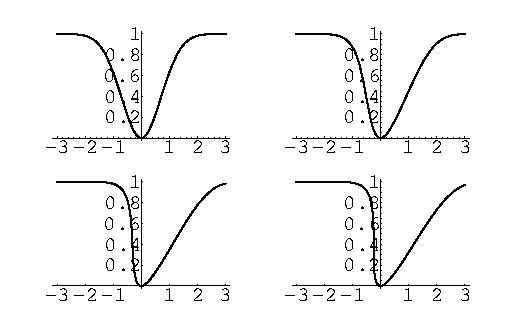
\includegraphics[width=0.5\textwidth]{nde/npde/burger1ex2}
      \end{center}
      \caption{The solution at various times.}
      \label{burger1ex2}
    \end{figure}
  \end{enumerate}
\end{Solution}








%%\phi_t + (1+x)\phi_x + \phi = 0 \quad \mathrm{in} \quad 
\begin{Solution}
  The method of characteristics gives us the differential equations
  \begin{alignat*}{2}
    x'(t) &= (1+x) &\qquad x(0) &= \xi \\
    \frac{\dd \phi}{\dd t} &= -\phi &\qquad \phi(\xi,0) &= f(\xi)
  \end{alignat*}
  Solving the first differential equation,
  \begin{gather*}
    x(t) = c e^{t} - 1, \qquad x(0) = \xi \\
    x(t) = (\xi+1)e^{t} - 1
  \end{gather*}
  The second differential equation then becomes
  \begin{gather*}
    \phi(x(t),t) = c e^{-t}, \qquad \phi(\xi,0) = f(\xi), \qquad
    \xi = (x+1)e^{-t} - 1 \\
    \phi(x,t) = f((x+1)e^{-t} - 1) e^{-t}
  \end{gather*}
  Thus the solution to the partial differential equation is
  \[ 
  \boxed{ 
    \phi(x,t) = f((x+1)e^{-t} - 1) e^{-t}. 
    } 
  \]
\end{Solution}



%%\phi_t + \phi_x + \frac{\alpha \phi}{1+x} = 0 
\begin{Solution}
  \[ \frac{\dd \phi}{\dd t} = \phi_t + x'(t) \phi_x = - \frac{\alpha \phi}{1+x} \]
  The characteristic curves $x(t)$ satisfy $x'(t) = 1$, so $x(t) = t + c$.
  The characteristic curve that separates the region with domain of 
  dependence on the $x$ axis and domain of dependence on  the $t$ axis is
  $x(t) = t$.  Thus we consider the two cases $x > t$ and $x < t$.
  \begin{itemize}
  \item $\mathbf{x > t}$.  $x(t) = t + \xi$.
  \item $\mathbf{x < t}$.  $x(t) = t - \tau$.
  \end{itemize}

  Now we solve the differential equation for $\phi$ in the two domains.
  \begin{itemize}
  \item $\mathbf{x > t}$.  
    \begin{gather*}
      \frac{\dd \phi}{\dd t} = -\frac{\alpha \phi}{1+x}, \qquad \phi(\xi,0)=0, \qquad
      \xi = x-t \\
      \frac{\dd \phi}{\dd t} = -\frac{\alpha \phi}{1+t+\xi} \\
      \phi = c \exp\left(-\alpha \int^t \frac{1}{t+\xi+1} \,d t \right) \\
      \phi = c exp\left(-\alpha \log(t+\xi+1) \right) \\
      \phi = c (t+\xi+1)^{-\alpha} \\
      \intertext{applying the initial condition, we see that}
      \phi = 0
    \end{gather*}
    %%
  \item $\mathbf{x < t}$.
    \begin{gather*}
      \frac{\dd \phi}{\dd t} = -\frac{\alpha \phi}{1+x}, \qquad \phi(0,\tau) = g(\tau),
      \qquad \tau = t-x \\
      \frac{\dd \phi}{\dd t} = - \frac{\alpha \phi}{1+t-\tau} \\
      \phi = c (t+1-\tau)^{-\alpha} \\
      \phi = g(\tau) (t+1-\tau)^{-\alpha} \\
      \phi = g(t-x) (x+1)^{-\alpha}
    \end{gather*}
  \end{itemize}
  Thus the solution to the partial differential equation is
  \[ \boxed{ \phi(x,t) = 
    \begin{cases}
      0 \quad &\mathrm{for}\ x > t \\
      g(t-x) (x+1)^{-\alpha} \quad &\mathrm{for}\ x < t.
    \end{cases}
    } \]
\end{Solution}



%%\phi_t + \phi_x +\phi^2 = 0 
\begin{Solution}
  The method of characteristics gives us the differential equations
  \begin{alignat*}{2}
    x'(t) &= 1 &\qquad x(0) &= \xi \\
    \frac{\dd \phi}{\dd t} &= -\phi^2 &\qquad \phi(\xi,0) &= f(\xi)
  \end{alignat*}
  Solving the first differential equation,
  \[ x(t) = t +\xi. \]
  The second differential equation is then
  \begin{gather*}
    \frac{\dd \phi}{\dd t} = -\phi^2, \qquad \phi(\xi,0) = f(\xi), \qquad
    \xi = x-t \\
    \phi^{-2} d\phi = - dt \\
    -\phi^{-1} = -t + c \\
    \phi = \frac{1}{t-c} \\
    \phi = \frac{1}{t + 1/f(\xi)} \\
    \boxed{ \phi = \frac{1}{t + 1/f(x-t)}. }
  \end{gather*}
\end{Solution}



%%c_t + c c_x + \mu c = 0, \qquad -\infty < x < \infty,\ t > 0 
\begin{Solution}
  \begin{enumerate}
    %%
    %%
    %%
  \item
    Taking the total derivative of $c$ with respect to $t$,
    \[ \frac{\dd c}{\dd t} = c_t + \frac{\dd x}{\dd t} c_x. \]
    Equating terms with the partial differential equation,
    we have the system of differential equations
    \begin{align*}
      \frac{\dd x}{\dd t} &= c \\
      \frac{\dd c}{\dd t} &= -\mu c.
    \end{align*}
    subject to the initial conditions
    \[ x(0) = \xi, \qquad c(\xi,0) = F(\xi). \]
    We can solve the second ODE directly.
    \begin{gather*}
      c(\xi,t) = c_1 e^{-\mu t} \\
      c(\xi,t) = F(\xi) e^{-\mu t}
    \end{gather*}
    Substituting this result and solving the first ODE,
    \begin{gather*}
      \frac{\dd x}{\dd t} = F(\xi) e^{-\mu t} \\
      x(t) = - \frac{F(\xi)}{\mu} e^{-\mu t} + c_2 \\
      x(t) = \frac{F(\xi)}{\mu}(1-e^{-\mu t}) + \xi.
    \end{gather*}

    The solution to the problem at the point $(x,t)$ is found by first solving
    \[ x = \frac{F(\xi)}{\mu}(1-e^{-\mu t}) + \xi \]
    for $\xi$ and then using this value to compute
    \[ c(x,t) = F(\xi) e^{-\mu t}. \]
    %%
    %%
    %%
  \item
    The characteristic lines are given by the equation
    \[ x(t) = \frac{F(\xi)}{\mu}(1-e^{-\mu t}) + \xi. \]
    The points on the envelope of characteristics also satisfy 
    \[ \frac{\partial x(t)}{\partial \xi} = 0. \]
    Thus the points on the envelope satisfy the system of equations
    \begin{align*}
      x &= \frac{F(\xi)}{\mu}(1-e^{-\mu t}) + \xi \\
      0 &= \frac{F'(\xi)}{\mu}(1-e^{-\mu t}) + 1.
    \end{align*}
    By substituting
    \[ 1-e^{-\mu t} = -\frac{\mu}{F'(\xi)} \]
    into the first equation we can eliminate its $t$ dependence.
    \[ x = -\frac{F(\xi)}{F'(\xi)} + \xi \]
    Now we can solve the second equation in the system for $t$.
    \begin{gather*}
      e^{-\mu t} = 1 + \frac{\mu}{F'(\xi)} \\
      t = -\frac{1}{\mu} \log\left(1 + \frac{\mu}{F'(\xi)} \right)
    \end{gather*}

    Thus the equations that describe the envelope are
    \begin{align*}
      x &= -\frac{F(\xi)}{F'(\xi)} + \xi \\
      t &= -\frac{1}{\mu} \log\left(1 + \frac{\mu}{F'(\xi)} \right).
    \end{align*}
    %%
    %%
    %%
  \item
    The second equation for the envelope has a solution for positive $t$ if
    there is some $x$ that satisfies
    \[ -1< \frac{\mu}{F'(x)} < 0. \]
    This is equivalent to
    \[ -\infty < F'(x) < -\mu. \]
    So in the case that $F'(x) < 0$, there will be breaking iff
    \[ \max |F'(x)| > \mu. \]
  \end{enumerate}
\end{Solution}



%%For water waves in a channel the so-called shallow water equations are
\begin{Solution}
  With the substitution $v = V(h)$, the two equations become
  \begin{gather*}
    h_t + (V + h V')h_x = 0 \\
    (V + h V')h_t + (V^2 + 2 h V V' + gh)h_x = 0.
  \end{gather*}
  We can rewrite the second equation as
  \[ h_t + \frac{V^2 + 2 h V V' + gh}{V + hV'} h_x = 0. \]
  Requiring that the two equations be consistent gives us a differential 
  equation for $V$.
  \begin{gather*}
    V + h V' = \frac{V^2 + 2 h V V' + gh}{V + hV'} \\
    V^2 + 2 h V V' + h^2 (V')^2 = V^2 + 2 h V V' + gh \\
    (V')^2 = \frac{g}{h}.
  \end{gather*}
  There are two choices depending on which sign we choose when taking the
  square root of the above equation.

  \textbf{Positive $\mathbf{V'}$.}
  \begin{gather*}
    V' = \sqrt{\frac{g}{h}} \\
    V = 2 \sqrt{g h} + \mathrm{const} \\
    \intertext{We apply the initial condition $V(h_0) = 0$.}
    \boxed{ V = 2 \sqrt{g}(\sqrt{h} - \sqrt{h_0}) }
  \end{gather*}

  The partial differential equation for $h$ is then
  \begin{gather*}
    h_t + (2 \sqrt{g}(\sqrt{h} - \sqrt{h_0})h)_x = 0 \\
    \boxed{ h_t + \sqrt{g}(3 \sqrt{h} - 2 \sqrt{h_0}) h_x = 0}
  \end{gather*}
  The wave speed is
  \[ \boxed{ c(h) = \sqrt{g}(3 \sqrt{h} - 2 \sqrt{h_0}). } \]


  \textbf{Negative $\mathbf{V'}$.}
  \begin{gather*}
    V' = - \sqrt{\frac{g}{h}} \\
    V = - 2 \sqrt{g h} + \mathrm{const} \\
    \intertext{We apply the initial condition $V(h_0) = 0$.}
    \boxed{ V = 2 \sqrt{g}(\sqrt{h_0} - \sqrt{h}) }
  \end{gather*}

  The partial differential equation for $h$ is then
  \[ \boxed{ h_t + \sqrt{g}(2 \sqrt{h_0} - 3 \sqrt{h}) h_x = 0.} \]
  The wave speed is
  \[ \boxed{ c(h) = \sqrt{g}(2 \sqrt{h_0} - 3 \sqrt{h}). } \]
\end{Solution}



%%After a change of variables, the chemical exchange equations can be put
\begin{Solution}
  \begin{enumerate}
    %%
    %%
    %%
  \item
    Making the substitutions, $\rho=\rho(X)$, $\sigma=\sigma(X)$, $X=x-Ut$, the
    system of partial differential equations becomes
    \begin{gather*}
      -U \rho' + \sigma' = 0 \\
      -U \rho' = \alpha \sigma - \beta \rho - \gamma \rho \sigma.
    \end{gather*}
    Integrating the first equation yields
    \begin{gather*}
      -U \rho + \sigma = c \\
      \sigma = c + U \rho.
    \end{gather*}
    Now we substitute the expression for $\sigma$ into the second partial 
    differential equation.
    \begin{gather*}
      -U \rho' = \alpha(c+U\rho) - \beta \rho - \gamma \rho(c+U\rho) \\
      \rho' = - \alpha\left(\rho+\frac{c}{U}\right) + \frac{\beta}{U}\rho
      + \gamma \rho\left(\rho+\frac{c}{U}\right) \\
      \intertext{Thus $\rho(X)$ satisfies the ordinary differential equation}
      \boxed{ \rho' = \gamma \rho^2 + \left(\frac{\gamma c}{U} + \frac{\beta}{U}
          -\alpha \right) \rho - \frac{\alpha c}{U}. }
    \end{gather*}
    %%
    %%
    %%
  \item
    Assume that
    \begin{align*}
      \rho(X) &\to \rho_1\ \mathrm{as}\ X \to +\infty \\
      \rho(X) &\to \rho_2\ \mathrm{as}\ X \to -\infty \\
      \rho'(X) &\to 0\ \mathrm{as}\ X \to \pm \infty.
    \end{align*}
    Integrating the ordinary differential equation for $\rho$,
    \[ X = \int^\rho \frac{d\rho}{\gamma \rho^2 + \left(\frac{\gamma c}{U} 
        + \frac{\beta}{U}-\alpha \right) \rho - \frac{\alpha c}{U}}. \]
    We see that the roots of the denominator of the integrand must be $\rho_1$
    and $\rho_2$.  Thus we can write the ordinary differential equation for 
    $\rho(X)$ as
    \[ \rho'(X) = \gamma(\rho-\rho_1)(\rho-\rho_2) = \gamma \rho^2
    - \gamma(\rho_1+\rho_2)\rho + \gamma \rho_1\rho_2. \]
    Equating coefficients in the polynomial with the differential equation 
    for part 1, we obtain the two equations
    \[ - \frac{\alpha c}{U} = \gamma \rho_1\rho_2, \qquad
    \frac{\gamma c}{U} + \frac{\beta}{U} -\alpha 
    = - \gamma(\rho_1+\rho_2).\]
    Solving the first equation for $c$,
    \[ c = - \frac{U \gamma \rho_1 \rho_2}{\alpha}. \]
    Now we substitute the expression for $c$ into the second equation.
    \begin{gather*}
      -\frac{\gamma U \gamma \rho_1 \rho_2}{\alpha U} + \frac{\beta}{U} -\alpha
      = - \gamma(\rho_1+\rho_2) \\
      \frac{\beta}{U} = \alpha + \frac{\gamma^2 \rho_1 \rho_2}{\alpha}
      - \gamma(\rho_1 + \rho_2) \\
      \intertext{Thus we see that $U$ is}
      \boxed{ U = \frac{\alpha \beta}{\alpha^2 + \gamma^2 \rho_1 \rho_2 - 
          - \alpha \gamma(\rho_1+\rho_2)}. }
    \end{gather*}

    Since the quadratic polynomial in the ordinary differential equation for 
    $\rho(X)$ is convex, it is negative valued between its two roots.  Thus we
    see that
    \[ \boxed{ \frac{\dd \rho}{\dd X} < 0. } \]

    Using the expression for $\sigma$ that we obtained in part 1,
    \begin{align*}
      \frac{\sigma_2-\sigma_1}{\rho_2-\rho_1}
      &= \frac{c+U\rho_2 - (c+U\rho_1)}{\rho_2-\rho_1} \\
      &= U \frac{\rho_2-\rho_1}{\rho_2-\rho_1} \\
      &= U.
    \end{align*}




    Now let's return to the ordinary differential equation
    for $\rho(X)$
    \begin{gather*}
      \rho'(X) = \gamma(\rho-\rho_1)(\rho-\rho_2) \\
      X = \int^\rho \frac{d\rho}{\gamma(\rho-\rho_1)(\rho-\rho_2)} \\
      X = -\frac{1}{\gamma(\rho_2-\rho_1)} \int^\rho \left( \frac{1}{\rho-\rho_1}
        + \frac{1}{\rho_2-\rho} \right)\,d\rho \\
      X - X_0 = -\frac{1}{\gamma(\rho_2-\rho_1)} \ln\left(\frac{\rho-\rho_1}
        {\rho_2-\rho}\right) \\
      -\gamma(\rho_2-\rho_1)(X-X_0) = \ln\left(\frac{\rho-\rho_1}
        {\rho_2-\rho}\right) \\
      \frac{\rho-\rho_1}{\rho_2-\rho} = \exp\left(-\gamma(\rho_2-\rho_1)(X-X_0)
      \right) \\
      \rho-\rho_1 = (\rho_2-\rho)\exp\left(-\gamma(\rho_2-\rho_1)(X-X_0)\right) \\
      \rho\left[1 + \exp\left(-\gamma(\rho_2-\rho_1)(X-X_0)\right)\right]
      = \rho_1+\rho_2 \exp\left(-\gamma(\rho_2-\rho_1)(X-X_0)\right) \\
      \intertext{Thus we obtain a closed form solution for $\rho$}
      \boxed{ \rho = \frac{\rho_1+\rho_2 \exp\left(-\gamma(\rho_2-\rho_1)(X-X_0)
          \right)}{1 + \exp\left(-\gamma(\rho_2-\rho_1)(X-X_0)\right)} }
    \end{gather*}
  \end{enumerate}
\end{Solution}



%%Find solitary wave solutions for the following equations:
\begin{Solution}
  \begin{enumerate}
    %%
    %%
    %%
  \item
    \[\eta_t + \eta_x + 6 \eta \eta_x - \eta_{xxt} = 0 \]
    We make the substitution
    \[ \eta(x,t) = z(X), \qquad X = x - U t. \]
    \begin{gather*}
      (1-U)z' + 6 z z' + U z''' = 0 \\
      (1-U)z + 3 z^2 + U z'' = 0 \\
      \frac{1}{2}(1-U)z^2 + z^3 + \frac{1}{2} U (z')^2 = 0 \\
      (z')^2 = \frac{U-1}{U}z^2  -\frac{2}{U}z^3 \\
      z(X) = \frac{U-1}{2} \sech^2 \left(\frac{1}{2}\sqrt{\frac{U-1}{U}} X\right) \\
      \eta(x,t) = \frac{U-1}{2} \sech^2 \left(\frac{1}{2}\left(\sqrt{\frac{U-1}{U}} 
          x - \sqrt{(U-1)U} t\right)\right) 
    \end{gather*}

    The linearized equation is
    \[\eta_t + \eta_x - \eta_{xxt} = 0. \]
    Substituting $\eta = e^{-\alpha x + \beta t}$ into this equation yields
    \begin{gather*}
      \beta - \alpha - \alpha^2 \beta = 0 \\
      \beta = \frac{\alpha}{1-\alpha^2}.
    \end{gather*}

    We set 
    \[ \alpha^2 = \frac{U-1}{U}. \]
    $\beta$ is then
    \begin{align*}
      \beta &= \frac{\alpha}{1-\alpha^2} \\
      &= \frac{\sqrt{(U-1)/U}}{1-(U-1)/U)} \\
      &= \frac{\sqrt{(U-1)U}}{U-(U-1)} \\
      &= \sqrt{(U-1)U}.
    \end{align*}

    The solution for $\eta$ becomes
    \[\frac{\alpha\beta}{2} \sech^2\left( \frac{\alpha x - \beta t}{2} \right)\]
    where
    \[ \beta = \frac{\alpha}{1-\alpha^2}. \]
    %%
    %%
    %%
  \item
    \[u_{tt} - u_{xx} - \left(\frac{3}{2} u^2\right)_{xx} - u_{xxxx}=0\]
    We make the substitution 
    \[ u(x,t) = z(X), \qquad X = x-Ut. \]
    \begin{gather*}
      (U^2-1)z'' - \left(\frac{3}{2} z^2\right)'' - z'''' = 0 \\
      (U^2-1)z' - \left(\frac{3}{2}z^2\right)' - z''' = 0 \\
      (U^2-1)z - \frac{3}{2}z^2 - z'' = 0 \\
      \intertext{We multiply by $z'$ and integrate.}
      \frac{1}{2}(U^2-1)z^2 - \frac{1}{2}z^3 - \frac{1}{2}(z')^2 = 0 \\
      (z')^2 = (U^2-1)z^2 - z^3 \\
      z = (U^2-1) \sech^2\left(\frac{1}{2}\sqrt{U^2-1}X\right) \\
      u(x,t) = (U^2-1) \sech^2\left(\frac{1}{2}\left(\sqrt{U^2-1} x
          - U \sqrt{U^2-1} t\right)\right)
    \end{gather*}

    The linearized equation is
    \[u_{tt} - u_{xx} - u_{xxxx}=0.\]
    Substituting $u = e^{-\alpha x + \beta t}$ into this equation yields
    \begin{gather*}
      \beta^2 - \alpha^2 - \alpha^4 = 0 \\
      \beta^2 = \alpha^2(\alpha^2+1).
    \end{gather*}

    We set
    \[ \alpha = \sqrt{U^2-1}. \]
    $\beta$ is then
    \begin{align*}
      \beta^2 &= \alpha^2(\alpha^2+1) \\
      &= (U^2-1)U^2 \\
      \beta &= U \sqrt{U^2-1}.
    \end{align*}

    The solution for $u$ becomes
    \[ u(x,t) = \alpha^2 \sech^2 \left(\frac{\alpha x - \beta t}{2}\right) \]
    where
    \[ \beta^2 = \alpha^2(\alpha^2+1). \]
    %%
    %%
    %%
  \item
    \[\phi_{tt} - \phi_{xx} + 2 \phi_x \phi_{xt} + \phi_{xx} \phi_t - \phi_{xxxx}\]
    We make the substitution 
    \[\phi(x,t) = z(X), \qquad X = x-Ut. \]
    \begin{gather*}
      (U^2-1)z'' - 2 U z' z'' - U z'' z' - z'''' = 0 \\
      (U^2-1)z'' - 3 U z' z'' - z'''' = 0 \\
      (U^2-1)z' - \frac{3}{2} (z')^2 - z''' = 0 \\
      \intertext{Multiply by $z''$ and integrate.}
      \frac{1}{2}(U^2-1)(z')^2 - \frac{1}{2} (z')^3 - \frac{1}{2} (z'')^2 = 0 \\
      (z'')^2 = (U^2-1)(z')^2 - (z')^3 \\
      z' = (U^2-1) \sech^2\left(\frac{1}{2} \sqrt{U^2-1} X\right) \\
      \phi_x(x,t) = (U^2-1) \sech^2\left(\frac{1}{2}\left( \sqrt{U^2-1}x
          - U \sqrt{U^2-1} t \right) \right).
    \end{gather*}


    The linearized equation is
    \[\phi_{tt} - \phi_{xx} - \phi_{xxxx}\]
    Substituting $\phi = e^{-\alpha x + \beta t}$ into this equation yields
    \[ \beta^2 = \alpha^2(\alpha^2+1). \]

    The solution for $\phi_x$ becomes
    \[ \phi_x = \alpha^2 \sech^2\left(\frac{\alpha x - \beta t}{2} \right) \]
    where
    \[ \beta^2 = \alpha^2(\alpha^2+1). \]
    %%
    %%
    %%
  \item
    \[u_t + 30 u^2 u_1 + 20 u_1 u_2 + 10 u u_3 + u_5 = 0 \]
    We make the substitution
    \[ u(x,t) = z(X), \qquad X=x-Ut. \]
    \begin{gather*}
      -Uz' + 30 z^2 z' + 20 z' z'' + 10 z z''' + z^{(5)} = 0 \\
      \intertext{Note that $(z z'')' = z'z'' + z z'''$.}
      -Uz' + 30 z^2 z' + 10 z' z'' + 10 (z z'')' + z^{(5)} = 0 \\
      -Uz + 10 z^3 + 5 (z')^2 + 10 z z'' + z^{(4)} = 0 \\
      \intertext{Multiply by $z'$ and integrate.}
      -\frac{1}{2} U z^2 + \frac{5}{2} z^4 + 5 z (z')^2 - \frac{1}{2} (z'')^2
      + z' z''' = 0 
    \end{gather*}

    Assume that
    \[ (z')^2 = P(z). \]
    Differentiating this relation,
    \begin{align*}
      2 z' z'' &= P'(z) z' \\
      z'' &= \frac{1}{2} P'(z) \\
      z''' &= \frac{1}{2} P''(z) z' \\
      z''' z' &= \frac{1}{2} P''(z) P(z).
    \end{align*}

    Substituting this expressions into the differential equation for $z$,
    \begin{gather*}
      -\frac{1}{2} U z^2 + \frac{5}{2} z^4 + 5 z P(z) - \frac{1}{2} \frac{1}{4}
      (P'(z))^2 + \frac{1}{2} P''(z) P(z) = 0 \\
      4 U z^2 + 20 z^4 + 40 z P(z) - (P'(z))^2 + 4 P''(z) P(z) = 0 \\
      \intertext{Substituting $P(z) = a z^3 + b z^2$ yields}
      (20 + 40 a + 15 a^2) z^4 + (40 b + 20 a b) z^3 + 
      (4b^2 + 4 U)z^2 = 0 
    \end{gather*}
    This equation is satisfied by $b^2 = U$, $a = -2$.  Thus we have
    \begin{gather*}
      (z')^2 = \sqrt{U} z^2 - 2 z^3 \\
      z = \frac{\sqrt{U}}{2} \sech^2 \left( \frac{1}{2} U^{1/4} X \right) \\
      u(x,t) = \frac{\sqrt{U}}{2} \sech^2 \left( \frac{1}{2} (U^{1/4} x 
        - U^{5/4} t) \right)
    \end{gather*}

    The linearized equation is
    \[u_t + u_5 = 0. \]
    Substituting $u = e^{-\alpha x + \beta t}$ into this equation yields
    \[ \beta - \alpha^5 = 0. \]
    We set 
    \[ \alpha = U^{1/4}. \]
    The solution for $u(x,t)$ becomes
    \[ \frac{\alpha^2}{2} \sech^2\left( \frac{\alpha x - \beta t}{2} \right) \]
    where 
    \[ \beta = \alpha^5. \]
  \end{enumerate}
\end{Solution}






\raggedbottom







